
%(BEGIN_QUESTION)
% Copyright 2012, Tony R. Kuphaldt, released under the Creative Commons Attribution License (v 1.0)
% This means you may do almost anything with this work of mine, so long as you give me proper credit

Suppose a radio transmitter sends 0.75 watts of power into one end of a twin-lead cable, the other end connected to an antenna.  The cable is 20 feet long, and exhibits a power loss of $-0.033$ dB/foot.  Calculate the power received by the antenna, in both units of watts and units of dBm.

\vskip 10pt

$P_{antenna}$ = \underbar{\hskip 50pt} watts

\vskip 10pt

$P_{antenna}$ = \underbar{\hskip 50pt} dBm

\vskip 20pt \vbox{\hrule \hbox{\strut \vrule{} {\bf Suggestions for Socratic discussion} \vrule} \hrule}

\begin{itemize}
\item{} A technique highly recommended for word-problems is to {\it sketch a picture} of the problem and label elements of that picture with the given information.  Do this, and compare your sketch with those of your classmates.  How, specifically, does this aid your problem-solving?
\item{} Solve this problem more than one way, and explain how these multiple solutions work.
\item{} Explain what ``dBm'' actually {\it means}.  Simple numerical examples may be helpful here:
\begin{itemize}

\item{} How much power is +3 dBm?
\item{} How much power is $-3$ dBm?
\item{} How much power is +10 dBm?
\item{} How much power is $-10$ dBm?
\end{itemize}
\end{itemize}

\underbar{file i01204}
%(END_QUESTION)





%(BEGIN_ANSWER)

$P_{antenna}$ = \underbar{\bf 0.644} watts

\vskip 10pt

$P_{antenna}$ = \underbar{\bf 28.09} dBm

%(END_ANSWER)





%(BEGIN_NOTES)

Sketching a picture of the problem is strongly recommended as a problem-solving technique:

$$\includegraphics[width=15.5cm]{i01204x01.eps}$$

The cable's loss of $-0.033$ dB per foot, over a 20 foot length, results in a total loss of $-0.66$ dB.  This equates to a power {\it ratio} of 0.8590 (i.e. only 85.90\% of the power output by the transmitter makes it to the antenna).  Thus, the power received by the antenna is:

$$(0.75 \hbox{ W})(0.8590) = 0.64426 \hbox{ W}$$

We could at this point convert 0.64426 watts into a dBm figure to arrive at the second answer (28.091 dBm), but for illustrative purposes let us do the whole problem again a different way.

\vskip 10pt

We may re-approach the problem by first expressing the transmitter's output power as a figure in dBm (0.75 W = 28.751 dBm).  Now, we may simply subtract the cable's loss (in units of dB) to arrive at the power seen at the antenna input:

$$28.751 \hbox{ dBm} - 0.66 \hbox{ dB} = 28.091 \hbox{ dBm}$$


\vfil \eject

\noindent
{\bf Prep Quiz:}

Suppose a radio transmitter sends 2 watts of power into one end of a twin-lead cable, the other end connected to an antenna.  The cable is 25 feet long, and exhibits a power loss of $-0.033$ dB/foot.  Calculate the power received by the antenna, in the unit of watts.

\begin{itemize}
\item{} 1.175 watts
\vskip 5pt 
\item{} 1.854 watts
\vskip 5pt 
\item{} 24.93 watts
\vskip 5pt 
\item{} 1.654 watts
\vskip 5pt 
\item{} 0.825 watts
\vskip 5pt 
\item{} 1.967 watts
\end{itemize}


\vfil \eject

\noindent
{\bf Prep Quiz:}

Suppose a radio transmitter sends 2.5 watts of power into one end of a coaxial cable, the other end connected to an antenna.  The cable is 20 feet long, and exhibits a power loss of $-0.017$ dB/foot.  Calculate the power received by the antenna, in the unit of watts.

\begin{itemize}
\item{} 2.312 watts
\vskip 5pt 
\item{} 2.167 watts
\vskip 5pt 
\item{} 1.577 watts
\vskip 5pt 
\item{} 2.404 watts
\vskip 5pt 
\item{} 2.160 watts
\vskip 5pt 
\item{} 2.483 watts
\end{itemize}


%INDEX% Electronics review: decibel power calculations

%(END_NOTES)


